\chapter{Pohlepni algoritmi}

\index{pohlepni algoritam}

\key{Pohlepni algoritam}
konstruira rješenje zadatka
tako da uvijek donosi odluku koja
u tom trenutku izgleda najbolje.
Pohlepni algoritam nikada ne poništava
svoje odluke, nego izravno konstruira
konačno rješenje.
Zbog toga su pohlepni algoritmi
obično vrlo efikasni.

Poteškoća u osmišljavanju pohlepnih algoritama
jest pronaći pohlepnu strategiju
koja uvijek daje optimalno rješenje
zadatka.
Lokalno optimalne odluke u pohlepnom
algoritmu trebale bi biti i globalno optimalne.
Često je teško argumentirati da
pohlepni algoritam radi ispravno.

\section{Zadatak s kovanicama}

Kao prvi primjer razmotrimo zadatak
u kojem nam je dan skup kovanica,
a zadatak nam je sastaviti novčani iznos $n$
pomoću tih kovanica.
Vrijednosti kovanica su
$\texttt{coins}=\{c_1,c_2,\ldots,c_k\}$,
a svaku kovanicu možemo upotrijebiti koliko puta želimo.
Koji je najmanji potreban broj kovanica?

Na primjer, ako su kovanice euro kovanice (u centima)
\[\{1,2,5,10,20,50,100,200\}\]
i $n=520$,
potrebne su nam barem četiri kovanice.
Optimalno rješenje je odabrati kovanice
$200+200+100+20$ čija je suma 520.

\subsubsection{Pohlepni algoritam}

Jednostavan pohlepni algoritam za ovaj zadatak
uvijek odabire najveću moguću kovanicu,
dok se traženi novčani iznos ne sastavi.
Taj algoritam radi u našem primjeru,
jer prvo odabiremo dvije kovanice od 200 centa,
zatim jednu kovanicu od 100 centa i naposljetku jednu od 20 centa.
No radi li taj algoritam uvijek?

Pokazuje se da, ako su kovanice euro kovanice,
pohlepni algoritam radi \emph{uvijek}, tj.
uvijek daje rješenje s najmanjim
mogućim brojem kovanica.
Ispravnost algoritma može se
pokazati na sljedeći način:

Prvo, svaka od kovanica 1, 5, 10, 50 i 100 pojavljuje se
najviše jednom u optimalnom rješenju,
jer kada bi
rješenje sadržavalo dvije takve kovanice,
mogli bismo ih zamijeniti jednom kovanicom i
dobiti bolje rješenje.
Na primjer, kada bi rješenje sadržavalo
kovanice $5+5$, mogli bismo ih zamijeniti kovanicom $10$.

Na isti način, kovanice 2 i 20 pojavljuju se
najviše dvaput u optimalnom rješenju,
jer bismo mogli zamijeniti
kovanice $2+2+2$ kovanicama $5+1$ i
kovanice $20+20+20$ kovanicama $50+10$.
Nadalje, optimalno rješenje ne može sadržavati
kovanice $2+2+1$ ni $20+20+10$,
jer bismo ih mogli zamijeniti kovanicama $5$ i $50$.

Koristeći ta zapažanja,
za svaku kovanicu $x$ možemo pokazati da
nije moguće optimalno sastaviti
iznos $x$ ni bilo koji veći iznos koristeći samo kovanice
manje od $x$.
Na primjer, ako je $x=100$, najveći optimalni
iznos pomoću manjih kovanica je  $50+20+20+5+2+2=99$.
Dakle, pohlepni algoritam koji uvijek odabire
najveću kovanicu daje optimalno rješenje.

Ovaj primjer pokazuje da može biti teško
argumentirati da pohlepni algoritam radi ispravno,
čak i ako je sam algoritam jednostavan.

\subsubsection{Opći slučaj}

U općem slučaju skup kovanica može sadržavati bilo kakve kovanice
i pohlepni algoritam \emph{ne} daje nužno
optimalno rješenje.

Da pohlepni algoritam ne radi ispravno možemo dokazati
tako da pokažemo protuprimjer
u kojem algoritam daje pogrešan odgovor.
U ovom zadatku lako nalazimo protuprimjer:
ako su kovanice $\{1,3,4\}$ a traženi iznos
je 6, pohlepni algoritam daje rješenje
$4+1+1$, dok je optimalno rješenje $3+3$.

Nije poznato može li se opći zadatak s kovanicama
riješiti bilo kakvim pohlepnim algoritmom\footnote{Ipak, moguće je
u polinomnom vremenu \emph{provjeriti}
radi li pohlepni algoritam predstavljen u ovom poglavlju za
zadani skup kovanica \cite{pea05}.}.
Međutim, kao što ćemo vidjeti u poglavlju 7,
u nekim slučajevima
opći se zadatak može efikasno
riješiti algoritmom dinamičkog
programiranja koji uvijek daje
ispravan odgovor.

\section{Raspoređivanje}

Mnogi se zadaci raspoređivanja mogu riješiti
pomoću pohlepnih algoritama.
Klasičan zadatak je sljedeći:
Dano je $n$ događaja s vremenima početka i završetka,
a treba pronaći raspored
koji uključuje što više događaja.
Nije moguće odabrati događaj djelomično.
Na primjer, razmotrimo sljedeće događaje:
\begin{center}
\begin{tabular}{lll}
događaj & vrijeme početka & vrijeme završetka \\
\hline
$A$ & 1 & 3 \\
$B$ & 2 & 5 \\
$C$ & 3 & 9 \\
$D$ & 6 & 8 \\
\end{tabular}
\end{center}
U ovom slučaju najveći broj događaja je dva.
Na primjer, možemo odabrati događaje $B$ i $D$
kako slijedi:
\begin{center}
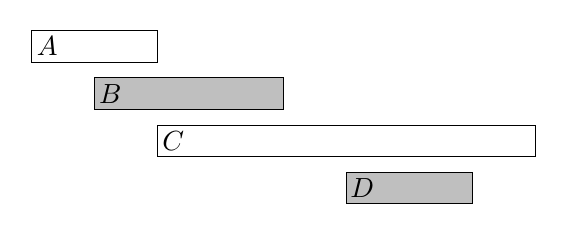
\begin{tikzpicture}[scale=.4]
  \begin{scope}
    \draw (2, 0) rectangle (6, -1);
    \draw[fill=lightgray] (4, -1.5) rectangle (10, -2.5);
    \draw (6, -3) rectangle (18, -4);
    \draw[fill=lightgray] (12, -4.5) rectangle (16, -5.5);
    \node at (2.5,-0.5) {$A$};
    \node at (4.5,-2) {$B$};
    \node at (6.5,-3.5) {$C$};
    \node at (12.5,-5) {$D$};
  \end{scope}
\end{tikzpicture}
\end{center}

Za ovaj zadatak moguće je osmisliti nekoliko pohlepnih algoritama,
no koji od njih radi u svakom slučaju?

\subsubsection*{Algoritam 1}

Prva je ideja odabirati što \emph{kraće}
događaje.
U našem primjeru taj algoritam
odabire sljedeće događaje:
\begin{center}
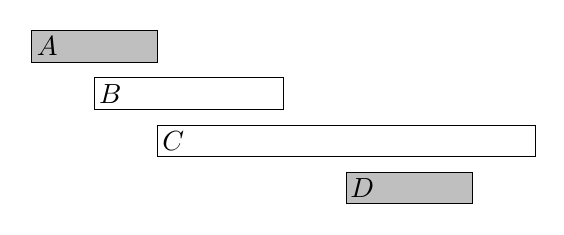
\begin{tikzpicture}[scale=.4]
  \begin{scope}
    \draw[fill=lightgray] (2, 0) rectangle (6, -1);
    \draw (4, -1.5) rectangle (10, -2.5);
    \draw (6, -3) rectangle (18, -4);
    \draw[fill=lightgray] (12, -4.5) rectangle (16, -5.5);
    \node at (2.5,-0.5) {$A$};
    \node at (4.5,-2) {$B$};
    \node at (6.5,-3.5) {$C$};
    \node at (12.5,-5) {$D$};
  \end{scope}
\end{tikzpicture}
\end{center}

Međutim, odabiranje kratkih događaja nije uvijek
ispravna strategija. Na primjer, algoritam ne uspijeva
u sljedećem slučaju:
\begin{center}
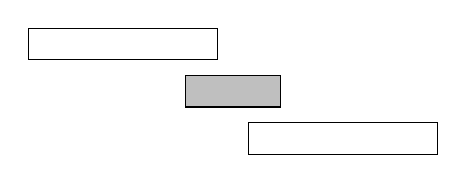
\begin{tikzpicture}[scale=.4]
  \begin{scope}
    \draw (1, 0) rectangle (7, -1);
    \draw[fill=lightgray] (6, -1.5) rectangle (9, -2.5);
    \draw (8, -3) rectangle (14, -4);
  \end{scope}
\end{tikzpicture}
\end{center}
Ako odaberemo kratki događaj, možemo odabrati samo jedan događaj.
Međutim, bilo bi moguće odabrati oba duga događaja.

\subsubsection*{Algoritam 2}

Druga je ideja uvijek odabrati sljedeći mogući
događaj koji \emph{počinje} što \emph{ranije}.
Taj algoritam odabire sljedeće događaje:
\begin{center}
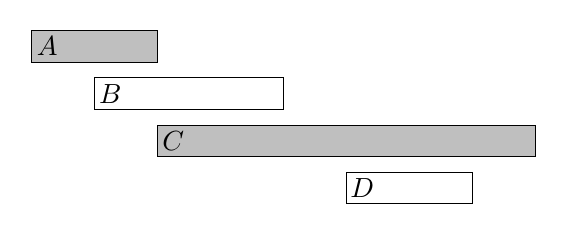
\begin{tikzpicture}[scale=.4]
  \begin{scope}
    \draw[fill=lightgray] (2, 0) rectangle (6, -1);
    \draw (4, -1.5) rectangle (10, -2.5);
    \draw[fill=lightgray] (6, -3) rectangle (18, -4);
    \draw (12, -4.5) rectangle (16, -5.5);
    \node at (2.5,-0.5) {$A$};
    \node at (4.5,-2) {$B$};
    \node at (6.5,-3.5) {$C$};
    \node at (12.5,-5) {$D$};
  \end{scope}
\end{tikzpicture}
\end{center}

Međutim, protuprimjer možemo naći
i za taj algoritam.
Na primjer, u sljedećem slučaju
algoritam odabire samo jedan događaj:
\begin{center}
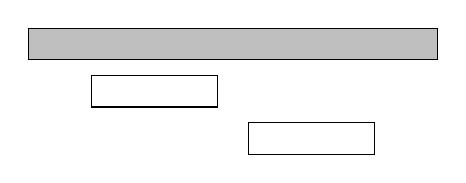
\begin{tikzpicture}[scale=.4]
  \begin{scope}
    \draw[fill=lightgray] (1, 0) rectangle (14, -1);
    \draw (3, -1.5) rectangle (7, -2.5);
    \draw (8, -3) rectangle (12, -4);
  \end{scope}
\end{tikzpicture}
\end{center}
Ako odaberemo prvi događaj, nije moguće
odabrati nijedan drugi događaj.
Međutim, bilo bi moguće odabrati
druga dva događaja.

\subsubsection*{Algoritam 3}

Treća je ideja uvijek odabrati sljedeći
mogući događaj koji \emph{završava} što \emph{ranije}.
Taj algoritam odabire sljedeće događaje: 
\begin{center}
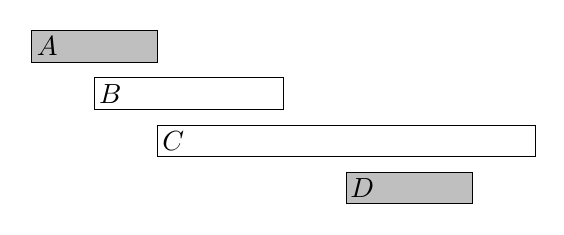
\begin{tikzpicture}[scale=.4]
  \begin{scope}
    \draw[fill=lightgray] (2, 0) rectangle (6, -1);
    \draw (4, -1.5) rectangle (10, -2.5);
    \draw (6, -3) rectangle (18, -4);
    \draw[fill=lightgray] (12, -4.5) rectangle (16, -5.5);
    \node at (2.5,-0.5) {$A$};
    \node at (4.5,-2) {$B$};
    \node at (6.5,-3.5) {$C$};
    \node at (12.5,-5) {$D$};
  \end{scope}
\end{tikzpicture}
\end{center}

Pokazuje se da taj algoritam
\emph{uvijek} daje optimalno rješenje.
Razlog je to što je uvijek optimalan odabir
prvo odabrati događaj koji završava
što ranije.
Nakon toga je optimalan odabir
odabrati sljedeći događaj
istom strategijom itd.,
dok više ne možemo odabrati nijedan događaj.

Jedan način da argumentiramo da algoritam radi
jest razmotriti
što se dogodi ako prvo odaberemo događaj
koji završava kasnije od događaja koji završava
što ranije.
Tada ćemo imati najviše jednak broj
mogućnosti za odabir sljedećeg događaja.
Stoga odabir događaja koji završava kasnije
nikada ne može dati bolje rješenje,
pa je pohlepni algoritam ispravan.

\section{Poslovi i rokovi}

Razmotrimo sada zadatak u kojem
nam je dano $n$ poslova s trajanjima i rokovima,
a naš je zadatak odabrati redoslijed obavljanja poslova.
Za svaki posao dobivamo $d-x$ bodova
gdje je $d$ rok posla
a $x$ trenutak u kojem dovršavamo posao.
Koji je najveći mogući ukupni rezultat
koji možemo postići?

Na primjer, pretpostavimo da su poslovi sljedeći:
\begin{center}
\begin{tabular}{lll}
posao & trajanje & rok \\
\hline
$A$ & 4 & 2 \\
$B$ & 3 & 5 \\
$C$ & 2 & 7 \\
$D$ & 4 & 5 \\
\end{tabular}
\end{center}
U ovom slučaju optimalan raspored poslova
je sljedeći:
\begin{center}
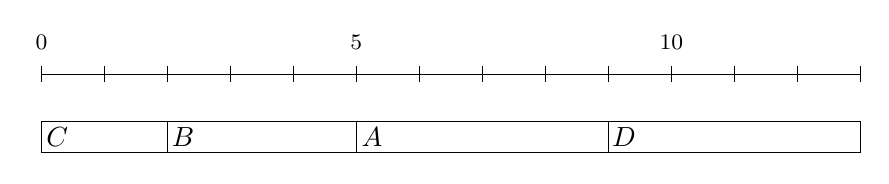
\begin{tikzpicture}[scale=.4]
  \begin{scope}
    \draw (0, 0) rectangle (4, -1);
    \draw (4, 0) rectangle (10, -1);
    \draw (10, 0) rectangle (18, -1);
    \draw (18, 0) rectangle (26, -1);
    \node at (0.5,-0.5) {$C$};
    \node at (4.5,-0.5) {$B$};
    \node at (10.5,-0.5) {$A$};
    \node at (18.5,-0.5) {$D$};

    \draw (0,1.5) -- (26,1.5);
    \foreach \i in {0,2,...,26}
    {
        \draw (\i,1.25) -- (\i,1.75);
    }
    \footnotesize
    \node at (0,2.5) {0};
    \node at (10,2.5) {5};
    \node at (20,2.5) {10};

  \end{scope}
\end{tikzpicture}
\end{center}
U tom rješenju $C$ daje 5 bodova,
$B$ daje 0 bodova, $A$ daje $-7$ bodova
a $D$ daje $-8$ bodova,
pa je ukupni rezultat $-10$.

Iznenađujuće, optimalno rješenje zadatka
uopće ne ovisi o rokovima,
nego je ispravna pohlepna strategija jednostavno
obavljati poslove \emph{sortirane po trajanju}
u rastućem redoslijedu.
Razlog je to što, ako ikada obavimo
dva posla jedan nakon drugoga tako da prvi posao
traje dulje od drugoga,
možemo dobiti bolje rješenje zamjenom tih poslova.
Na primjer, razmotrimo sljedeći raspored:
\begin{center}
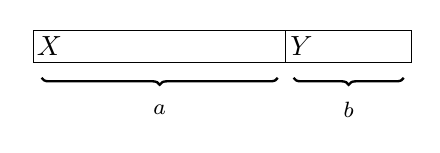
\begin{tikzpicture}[scale=.4]
  \begin{scope}
    \draw (0, 0) rectangle (8, -1);
    \draw (8, 0) rectangle (12, -1);
    \node at (0.5,-0.5) {$X$};
    \node at (8.5,-0.5) {$Y$};

\draw [decoration={brace}, decorate, line width=0.3mm] (7.75,-1.5) -- (0.25,-1.5);
\draw [decoration={brace}, decorate, line width=0.3mm] (11.75,-1.5) -- (8.25,-1.5);

\footnotesize
\node at (4,-2.5) {$a$};
\node at (10,-2.5) {$b$};

  \end{scope}
\end{tikzpicture}
\end{center}
Ovdje je $a>b$, pa bismo trebali zamijeniti poslove:
\begin{center}
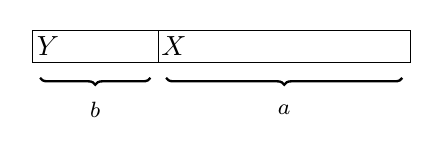
\begin{tikzpicture}[scale=.4]
  \begin{scope}
    \draw (0, 0) rectangle (4, -1);
    \draw (4, 0) rectangle (12, -1);
    \node at (0.5,-0.5) {$Y$};
    \node at (4.5,-0.5) {$X$};

\draw [decoration={brace}, decorate, line width=0.3mm] (3.75,-1.5) -- (0.25,-1.5);
\draw [decoration={brace}, decorate, line width=0.3mm] (11.75,-1.5) -- (4.25,-1.5);

\footnotesize
\node at (2,-2.5) {$b$};
\node at (8,-2.5) {$a$};

  \end{scope}
\end{tikzpicture}
\end{center}
Sada $X$ daje $b$ bodova manje a $Y$ daje $a$ bodova više,
pa se ukupni rezultat povećava za $a-b > 0$.
U optimalnom rješenju
za svaka dva uzastopna posla
mora vrijediti da kraći posao dolazi
prije duljeg posla.
Dakle, poslovi se moraju obavljati
sortirani po svojim trajanjima.

\section{Minimiziranje suma}

Zatim razmatramo zadatak u kojem
nam je dano $n$ brojeva $a_1,a_2,\ldots,a_n$
a naš je zadatak pronaći vrijednost $x$
koja minimizira sumu
\[|a_1-x|^c+|a_2-x|^c+\cdots+|a_n-x|^c.\]
Usredotočujemo se na slučajeve $c=1$ i $c=2$.

\subsubsection{Slučaj $c=1$}

U ovom slučaju trebamo minimizirati sumu
\[|a_1-x|+|a_2-x|+\cdots+|a_n-x|.\]
Na primjer, ako su brojevi $[1,2,9,2,6]$,
najbolje je rješenje odabrati $x=2$
što daje sumu
\[
|1-2|+|2-2|+|9-2|+|2-2|+|6-2|=12.
\]
U općem slučaju najbolji odabir za $x$
je \textit{medijan} brojeva,
tj. srednji broj nakon sortiranja.
Na primjer, lista $[1,2,9,2,6]$
nakon sortiranja postaje $[1,2,2,6,9]$,
pa je medijan 2.

Medijan je optimalan odabir,
jer ako je $x$ manji od medijana,
suma se smanjuje povećavanjem $x$,
a ako je $x$ veći od medijana,
suma se smanjuje smanjivanjem $x$.
Stoga je optimalno rješenje da je $x$
medijan.
Ako je $n$ paran i postoje dva medijana,
oba medijana i sve vrijednosti između njih
optimalni su odabiri.

\subsubsection{Slučaj $c=2$}

U ovom slučaju trebamo minimizirati sumu
\[(a_1-x)^2+(a_2-x)^2+\cdots+(a_n-x)^2.\]
Na primjer, ako su brojevi $[1,2,9,2,6]$,
najbolje je rješenje odabrati $x=4$
što daje sumu
\[
(1-4)^2+(2-4)^2+(9-4)^2+(2-4)^2+(6-4)^2=46.
\]
U općem slučaju najbolji odabir za $x$
je \emph{prosjek} brojeva.
U našem primjeru prosjek je $(1+2+9+2+6)/5=4$.
Taj se rezultat može izvesti prikazivanjem
sume na sljedeći način:
\[
nx^2 - 2x(a_1+a_2+\cdots+a_n) + (a_1^2+a_2^2+\cdots+a_n^2)
\]
Posljednji dio ne ovisi o $x$,
pa ga možemo zanemariti.
Preostali dijelovi tvore funkciju
$nx^2-2xs$ gdje je $s=a_1+a_2+\cdots+a_n$.
To je parabola otvorena prema gore
s nultočkama $x=0$ i $x=2s/n$,
a minimalna vrijednost je prosjek
nultočaka $x=s/n$, tj.
prosjek brojeva $a_1,a_2,\ldots,a_n$.

\section{Kompresija podataka}

\index{kompresija podataka}
\index{binarni kod}
\index{kodna riječ}

\key{Binarni kod} svakom znaku
znakovnog niza dodjeljuje \key{kodnu riječ} koja se sastoji od bitova.
Znakovni niz možemo \emph{komprimirati} pomoću binarnog koda
tako da svaki znak zamijenimo
odgovarajućom kodnom riječju.
Na primjer, sljedeći binarni kod
dodjeljuje kodne riječi znakovima
\texttt{A}–\texttt{D}:
\begin{center}
\begin{tabular}{rr}
znak & kodna riječ \\
\hline
\texttt{A} & 00 \\
\texttt{B} & 01 \\
\texttt{C} & 10 \\
\texttt{D} & 11 \\
\end{tabular}
\end{center}
To je kod \key{konstantne dužine}
što znači da je dužina svake
kodne riječi jednaka.
Na primjer, znakovni niz
\texttt{AABACDACA} možemo komprimirati kako slijedi:
\[00\,00\,01\,00\,10\,11\,00\,10\,00\]
Uz taj kod dužina komprimiranog
znakovnog niza je 18 bitova.
Međutim, znakovni niz možemo komprimirati bolje
ako upotrijebimo kod \key{varijabilne dužine}
u kojem kodne riječi mogu imati različite dužine.
Tada možemo dati kratke kodne riječi
znakovima koji se pojavljuju često
i duge kodne riječi znakovima
koji se pojavljuju rijetko.
Pokazuje se da je \key{optimalan} kod
za navedeni znakovni niz sljedeći:
\begin{center}
\begin{tabular}{rr}
znak & kodna riječ \\
\hline
\texttt{A} & 0 \\
\texttt{B} & 110 \\
\texttt{C} & 10 \\
\texttt{D} & 111 \\
\end{tabular}
\end{center}
Optimalan kod daje komprimirani znakovni niz
koji je što kraći.
U ovom slučaju komprimirani znakovni niz uz
optimalan kod je
\[0\,0\,110\,0\,10\,111\,0\,10\,0,\]
pa je potrebno samo 15 bitova umjesto 18 bitova.
Dakle, zahvaljujući boljem kodu bilo je moguće
uštedjeti 3 bita u komprimiranom znakovnom nizu.

Zahtijevamo da nijedna kodna riječ
nije prefiks druge kodne riječi.
Na primjer, nije dopušteno da kod
sadrži i kodnu riječ 10
i kodnu riječ 1011.
Razlog je to što želimo
moći iz komprimiranog znakovnog niza
generirati izvorni znakovni niz.
Kada bi kodna riječ mogla biti prefiks druge kodne riječi,
to ne bi uvijek bilo moguće.
Na primjer, sljedeći kod \emph{nije} valjan:
\begin{center}
\begin{tabular}{rr}
znak & kodna riječ \\
\hline
\texttt{A} & 10 \\
\texttt{B} & 11 \\
\texttt{C} & 1011 \\
\texttt{D} & 111 \\
\end{tabular}
\end{center}
Uz taj kod ne bi bilo moguće znati
odgovara li komprimirani znakovni niz 1011
znakovnom nizu \texttt{AB} ili znakovnom nizu \texttt{C}.

\index{Huffmanovo kodiranje}

\subsubsection{Huffmanovo kodiranje}

\key{Huffmanovo kodiranje}\footnote{D. A. Huffman otkrio je tu metodu
rješavajući zadatak na sveučilišnom kolegiju
te je objavio algoritam 1952. \cite{huf52}.} je pohlepni algoritam
koji konstruira optimalan kod za
kompresiju zadanog znakovnog niza.
Algoritam gradi binarno stablo
na temelju frekvencija znakova
u znakovnom nizu,
a kodna riječ svakog znaka može se pročitati
prateći put od korijena do
odgovarajućeg čvora.
Pomak ulijevo odgovara bitu 0,
a pomak udesno odgovara bitu 1.

Na početku je svaki znak znakovnog niza
predstavljen čvorom čija je težina
broj pojavljivanja tog znaka u znakovnom nizu.
Zatim se u svakom koraku dva čvora s minimalnim težinama
spajaju stvaranjem
novog čvora čija je težina suma težina
izvornih čvorova.
Postupak se nastavlja dok svi čvorovi ne budu spojeni.

Sljedeće ćemo vidjeti kako Huffmanovo kodiranje stvara
optimalan kod za znakovni niz
\texttt{AABACDACA}.
Na početku postoje četiri čvora koji odgovaraju
znakovima znakovnog niza:

\begin{center}
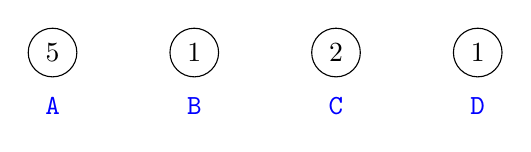
\begin{tikzpicture}[scale=0.9]
\node[draw, circle] (1) at (0,0) {$5$};
\node[draw, circle] (2) at (2,0) {$1$};
\node[draw, circle] (3) at (4,0) {$2$};
\node[draw, circle] (4) at (6,0) {$1$};

\node[color=blue] at (0,-0.75) {\texttt{A}};
\node[color=blue] at (2,-0.75) {\texttt{B}};
\node[color=blue] at (4,-0.75) {\texttt{C}};
\node[color=blue] at (6,-0.75) {\texttt{D}};

%\path[draw,thick,-] (4) -- (5);
\end{tikzpicture}
\end{center}
Čvor koji predstavlja znak \texttt{A}
ima težinu 5 jer se znak \texttt{A}
u znakovnom nizu pojavljuje 5 puta.
Ostale su težine izračunate
na isti način.

Prvi korak je spojiti čvorove koji
odgovaraju znakovima \texttt{B} i \texttt{D},
oba s težinom 1.
Rezultat je:
\begin{center}
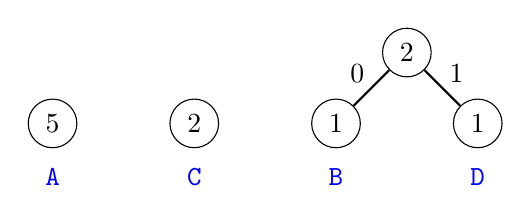
\begin{tikzpicture}[scale=0.9]
\node[draw, circle] (1) at (0,0) {$5$};
\node[draw, circle] (3) at (2,0) {$2$};
\node[draw, circle] (2) at (4,0) {$1$};
\node[draw, circle] (4) at (6,0) {$1$};
\node[draw, circle] (5) at (5,1) {$2$};

\node[color=blue] at (0,-0.75) {\texttt{A}};
\node[color=blue] at (2,-0.75) {\texttt{C}};
\node[color=blue] at (4,-0.75) {\texttt{B}};
\node[color=blue] at (6,-0.75) {\texttt{D}};

\node at (4.3,0.7) {0};
\node at (5.7,0.7) {1};

\path[draw,thick,-] (2) -- (5);
\path[draw,thick,-] (4) -- (5);
\end{tikzpicture}
\end{center}
Nakon toga spajaju se čvorovi s težinom 2:
\begin{center}
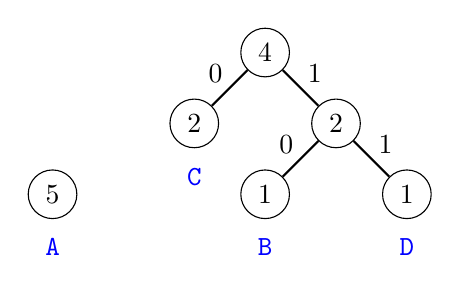
\begin{tikzpicture}[scale=0.9]
\node[draw, circle] (1) at (1,0) {$5$};
\node[draw, circle] (3) at (3,1) {$2$};
\node[draw, circle] (2) at (4,0) {$1$};
\node[draw, circle] (4) at (6,0) {$1$};
\node[draw, circle] (5) at (5,1) {$2$};
\node[draw, circle] (6) at (4,2) {$4$};

\node[color=blue] at (1,-0.75) {\texttt{A}};
\node[color=blue] at (3,1-0.75) {\texttt{C}};
\node[color=blue] at (4,-0.75) {\texttt{B}};
\node[color=blue] at (6,-0.75) {\texttt{D}};

\node at (4.3,0.7) {0};
\node at (5.7,0.7) {1};
\node at (3.3,1.7) {0};
\node at (4.7,1.7) {1};

\path[draw,thick,-] (2) -- (5);
\path[draw,thick,-] (4) -- (5);
\path[draw,thick,-] (3) -- (6);
\path[draw,thick,-] (5) -- (6);
\end{tikzpicture}
\end{center}
Naposljetku se spajaju dva preostala čvora:
\begin{center}
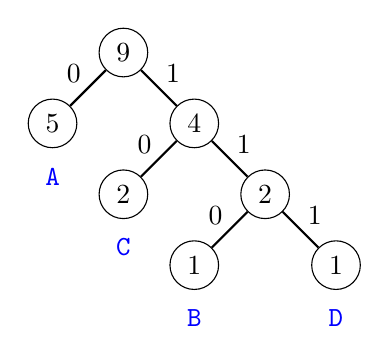
\begin{tikzpicture}[scale=0.9]
\node[draw, circle] (1) at (2,2) {$5$};
\node[draw, circle] (3) at (3,1) {$2$};
\node[draw, circle] (2) at (4,0) {$1$};
\node[draw, circle] (4) at (6,0) {$1$};
\node[draw, circle] (5) at (5,1) {$2$};
\node[draw, circle] (6) at (4,2) {$4$};
\node[draw, circle] (7) at (3,3) {$9$};

\node[color=blue] at (2,2-0.75) {\texttt{A}};
\node[color=blue] at (3,1-0.75) {\texttt{C}};
\node[color=blue] at (4,-0.75) {\texttt{B}};
\node[color=blue] at (6,-0.75) {\texttt{D}};

\node at (4.3,0.7) {0};
\node at (5.7,0.7) {1};
\node at (3.3,1.7) {0};
\node at (4.7,1.7) {1};
\node at (2.3,2.7) {0};
\node at (3.7,2.7) {1};

\path[draw,thick,-] (2) -- (5);
\path[draw,thick,-] (4) -- (5);
\path[draw,thick,-] (3) -- (6);
\path[draw,thick,-] (5) -- (6);
\path[draw,thick,-] (1) -- (7);
\path[draw,thick,-] (6) -- (7);
\end{tikzpicture}
\end{center}

Sada su svi čvorovi u stablu, pa je kod gotov.
Iz stabla se mogu pročitati sljedeće kodne riječi:
\begin{center}
\begin{tabular}{rr}
znak & kodna riječ \\
\hline
\texttt{A} & 0 \\
\texttt{B} & 110 \\
\texttt{C} & 10 \\
\texttt{D} & 111 \\
\end{tabular}
\end{center}
